\documentclass[border=1cm]{standalone}
\usepackage{tikz} 
\usepackage{framed}

\colorlet{tapeBg}{red!30}
\colorlet{tapeBorder}{red!60}

\tikzset{
nodestyle/.style={circle, minimum size=0pt, inner sep=0pt},
boxstyle/.style={rectangle, inner sep = 2pt, outer sep = 0pt, draw, fill=white}
}

% fresh posx posy
\newcommand{\id}[3]{
  \node [nodestyle] (ida#1) at (#2,#3) {};
  \node [nodestyle] (idb#1) at (#2 + 1,#3) {};
  \draw (ida#1) -- (idb#1);
}

% fresh posx posy scaley
\newcommand{\swap}[4]{
 \node [nodestyle] (swapa1) at (#2,#3) {};
 \node [nodestyle] (swapb1) at (#2,#3 + #4) {};
 \node [nodestyle] (swapc1) at (#2+1,#3) {};
 \node [nodestyle] (swapd1) at (#2+1,#3 + #4) {};
  
 \draw [in=180, out=0] (swapa1) to (swapd1);
 \draw [in=-180, out=0] (swapb1) to (swapc1);
}

% fresh posx posy arity-1 coarity-1 name otimesdist
\newcommand{\gen}[7]{
  \node [color=gray] () at (#2, #3) {$\bot$};
  \pgfmathsetmacro\arminone{#4};
  \pgfmathsetmacro\coarminone{#5};
  \pgfmathsetmacro\otimesdist{#7};

  \pgfmathsetmacro\arity{#4 + 1};
  \pgfmathsetmacro\coarity{#5 + 1};

\pgfmathparse{%
  (\arity>\coarity)
    ? \arminone * \otimesdist
    : \coarminone * \otimesdist
}%
\let\height\pgfmathresult


  \node [boxstyle] (a) at (#2 + 1,#3 + \height / 2) {#6};

  \pgfmathparse{%
  (\arity - 1) / 2 * \otimesdist
}%
\let\arshift\pgfmathresult

\pgfmathparse{%
  (\coarity - 1) / 2 * \otimesdist
  }%
\let\coarshift\pgfmathresult

   \foreach \i in {0,...,\arminone}
  {
    \node [nodestyle] (#1in\i) at (#2, #3 + \i * \otimesdist + \height / 2 - \arshift) {};

    % Correct conditional computation
     % Use TeX conditional to avoid division by zero
    \ifnum\arminone=0
      \def\angle{180}
    \else
      \pgfmathsetmacro{\angle}{(180 / \arminone) * -\i - 90}
    \fi

    \draw[in=0, out=\angle] (a) to (#1in\i);
  }

  \foreach \i in {0,...,\coarminone}
  {
    \node [nodestyle] (#1out\i) at (#2 + 2, #3 + \i * \otimesdist + \height / 2 - \coarshift) {};

    % Correct conditional computation
     % Use TeX conditional to avoid division by zero
    \ifnum\coarminone=0
      \def\angle{0}
    \else
      \pgfmathsetmacro{\angle}{(180 / \coarminone) * \i - 90}
    \fi

    \draw[in=180, out=\angle] (a) to (#1out\i);
  }
}


% posx posy width height
\newcommand{\tape}[4]{
  \draw [fill=tapeBg, tapeBg] (#1, #2) -- (#1+#3, #2) -- (#1+#3, #2+#4) -- (#1, #2+#4) -- cycle;
  
  \draw[tapeBorder, line width=0.5pt] (#1, #2) -- (#1+#3, #2);
  \draw[tapeBorder, line width=0.5pt] (#1+#3, #2+#4) -- (#1, #2+#4);
}

% posxll posyll posxlu posylu posxrl posyrl posxru posyru
\newcommand{\freestyletape}[8]{
  \draw [fill=tapeBg, tapeBg] (#1, #2) -- (#3, #4) [in=180, out=0] to (#7, #8) -- (#5, #6)  [in=0, out=180] to cycle;

   \draw[tapeBorder, line width=0.5pt, in=180, out=0] (#1, #2) to (#5, #6);
  \draw[tapeBorder, line width=0.5pt, in=180, out=0] (#3, #4) to (#7, #8);
}

% posx posy h1 h2 
\newcommand{\adapter}[4] {
  \draw [fill=tapeBg, tapeBg] (#1, #2 - #3 / 2) -- (#1, #2 + #3 / 2) -- (#1+0.5, #2+#4/2) -- (#1+0.5, #2 - #4 / 2) -- cycle;
}


% posx posy n1 n2 oplusdist otimesdist tapepadding width
\newcommand{\swaptape}[8]{
  \pgfmathsetmacro{\posx}{#1}
  \pgfmathsetmacro{\posy}{#2}
  \pgfmathsetmacro{\none}{#3}
  \pgfmathsetmacro{\ntwo}{#4}
  \pgfmathsetmacro{\oplusdist}{#5}
  \pgfmathsetmacro{\otimesdist}{#6}
  \pgfmathsetmacro{\tapepadding}{#7}
  \pgfmathsetmacro{\width}{#8}

   \ifnum\none=0
      \pgfmathsetmacro{\sizeone}{2 * \tapepadding}
    \else
      \pgfmathsetmacro{\sizeone}{(\none - 1) * \otimesdist + (2 * \tapepadding)}
    \fi

    \ifnum\ntwo=0
      \pgfmathsetmacro{\sizetwo}{2 * \tapepadding}
    \else
      \pgfmathsetmacro{\sizetwo}{(\ntwo - 1) * \otimesdist + (2 * \tapepadding)}
    \fi

    \pgfmathsetmacro{\twobasebotx}{\posx}
    \pgfmathsetmacro{\twobaseboty}{\posy}

    \pgfmathsetmacro{\twoceilbotx}{\posx}
    \pgfmathsetmacro{\twoceilboty}{\posy + \sizetwo}

    \pgfmathsetmacro{\twobasetopx}{\posx + \width}
    \pgfmathsetmacro{\twobasetopy}{\posy + \sizeone + \oplusdist}

    \pgfmathsetmacro{\twoceiltopx}{\posx + \width}
    \pgfmathsetmacro{\twoceiltopy}{\posy + \sizeone + \oplusdist + \sizetwo}

    \pgfmathsetmacro{\onebasebotx}{\posx + \width}
    \pgfmathsetmacro{\onebaseboty}{\posy}

    \pgfmathsetmacro{\oneceilbotx}{\posx + \width}
    \pgfmathsetmacro{\oneceilboty}{\posy + \sizeone}

    \pgfmathsetmacro{\onebasetopx}{\posx}
    \pgfmathsetmacro{\onebasetopy}{\posy + \sizetwo + \oplusdist}

    \pgfmathsetmacro{\oneceiltopx}{\posx}
    \pgfmathsetmacro{\oneceiltopy}{\posy + \sizetwo + \oplusdist + \sizeone}

    \draw [fill=tapeBg, tapeBg, in=180, out=0] (\twobasebotx, \twobaseboty) to (\twobasetopx, \twobasetopy) --  (\twoceiltopx, \twoceiltopy) [in=0, out=180] to (\twoceilbotx, \twoceilboty) -- cycle;

    \draw [fill=tapeBg, tapeBg, in=0, out=180] (\onebasebotx, \onebaseboty) to (\onebasetopx, \onebasetopy) --  (\oneceiltopx, \oneceiltopy) [in=180, out=0] to (\oneceilbotx, \oneceilboty) -- cycle;

    \draw[tapeBorder, in=180, out=0] (\twobasebotx, \twobaseboty) to (\twobasetopx, \twobasetopy);
    \draw[tapeBorder, in=180, out=0] (\twoceilbotx, \twoceilboty) to (\twoceiltopx, \twoceiltopy);


    \draw[tapeBorder, in=0, out=180] (\onebasebotx, \onebaseboty) to (\onebasetopx, \onebasetopy);
    \draw[tapeBorder, in=0, out=180] (\oneceilbotx, \oneceilboty) to (\oneceiltopx, \oneceiltopy);


    \foreach \i in {0,...,\ntwo}
    {
      \pgfmathsetmacro{\iminone}{\i - 1}
      \ifnum\i=0
    \else
      \draw[in=180, out=0] (\twobasebotx, \twobaseboty + \iminone * \otimesdist + \tapepadding) to (\twobasetopx, \twobasetopy + \iminone * \otimesdist + \tapepadding);
    \fi
    }

    \foreach \i in {0,...,\none}
    {
    \pgfmathsetmacro{\iminone}{\i - 1}
     \ifnum\i=0
    \else
      \draw[in=0, out=180] (\oneceilbotx, \onebaseboty + \iminone * \otimesdist + \tapepadding) to   (\onebasetopx, \onebasetopy + (\iminone * \otimesdist + \tapepadding);
    \fi



    }


}

% fresh name, len, posx, posy
\newcommand{\measuretape}[4]{
  \pgfmathsetmacro{\len}{#2 * 1}

  \node [nodestyle] (measa#1) at (#3,#4) {};
  \node [nodestyle] (measb#1) at (#3,#4+#2) {};
  \node [nodestyle] () at (#3,#4+#2+.3) {$\len$};
  \draw [|-|] (measa#1) -- (measb#1);
}
\begin{document}
 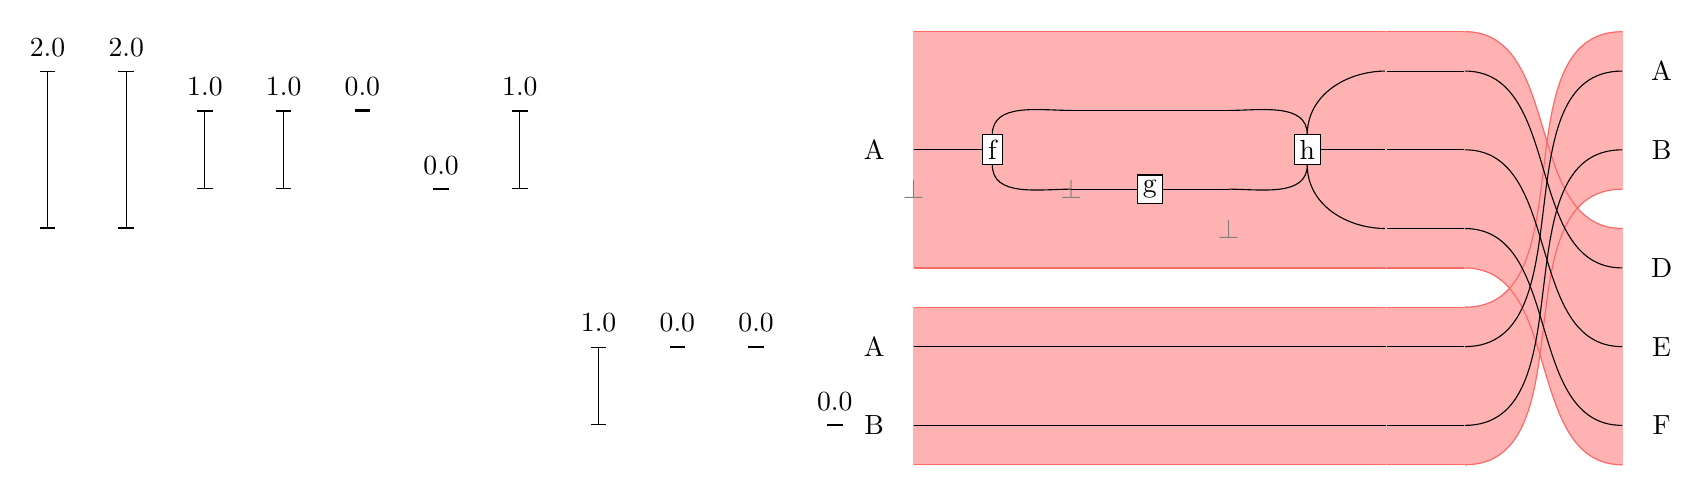
\begin{tikzpicture}[inner sep=0,outer sep=0]



 
\freestyletape {6.000000} {2.500000} {6.000000} {5.500000} {7.000000} {2.500000} {7.000000} {5.500000}\draw [in=180, out=0] (6.000000 , 5.000000) to (7.000000 , 5.000000);
\draw [in=180, out=0] (6.000000 , 4.000000) to (7.000000 , 4.000000);
\draw [in=180, out=0] (6.000000 , 3.000000) to (7.000000 , 3.000000);
\freestyletape {6.000000} {0.000000} {6.000000} {2.000000} {7.000000} {0.000000} {7.000000} {2.000000}\draw [in=180, out=0] (6.000000 , 1.500000) to (7.000000 , 1.500000);
\draw [in=180, out=0] (6.000000 , 0.500000) to (7.000000 , 0.500000);
\tape {0.000000} {2.500000} {6.000000} {3.000000}
\gen {1}{0.000000}{3.500000}{0}{1}{f}{1.000000}
\measuretape {5} {1.000000} {-5.000000} {3.500000}
\id{3}{2.000000}{4.500000}
\measuretape {7} {0.000000} {-7.000000} {4.500000}
\gen {2}{2.000000}{3.500000}{0}{0}{g}{1.000000}
\measuretape {6} {0.000000} {-6.000000} {3.500000}
% adjusting misaligned tensors:
\draw [in=180, out=0] (3.000000 , 4.500000) to (4.000000 , 4.500000);
\draw [in=180, out=0] (4.000000 , 3.500000) to (4.000000 , 3.500000);
\measuretape {8} {1.000000} {-8.000000} {3.500000}
% composing interfaces:
\draw [in=180, out=0] (2.000000 , 4.500000) to (2.000000 , 4.500000);
\draw [in=180, out=0] (2.000000 , 3.500000) to (2.000000 , 3.500000);
\measuretape {9} {1.000000} {-9.000000} {3.500000}
\gen {3}{4.000000}{3.000000}{1}{2}{h}{1.000000}
\measuretape {10} {2.000000} {-10.000000} {3.000000}
% composing interfaces:
\draw [in=180, out=0] (4.000000 , 4.500000) to (4.000000 , 4.500000);
\draw [in=180, out=0] (4.000000 , 3.500000) to (4.000000 , 3.500000);
\measuretape {11} {2.000000} {-11.000000} {3.000000}
\tape {0.000000} {0.000000} {1.000000} {2.000000}
\id{2}{0.000000}{1.500000}
\measuretape {2} {0.000000} {-2.000000} {1.500000}
\measuretape {3} {0.000000} {-3.000000} {1.500000}
\id{1}{0.000000}{0.500000}
\measuretape {1} {0.000000} {-1.000000} {0.500000}
% adjusting misaligned tensors:
\draw [in=180, out=0] (1.000000 , 1.500000) to (1.000000 , 1.500000);
\draw [in=180, out=0] (1.000000 , 0.500000) to (1.000000 , 0.500000);
\measuretape {4} {1.000000} {-4.000000} {0.500000}
\freestyletape {6.000000} {2.500000} {6.000000} {5.500000} {6.000000} {2.500000} {6.000000} {5.500000}\draw [in=180, out=0] (6.000000 , 5.000000) to (6.000000 , 5.000000);
\draw [in=180, out=0] (6.000000 , 4.000000) to (6.000000 , 4.000000);
\draw [in=180, out=0] (6.000000 , 3.000000) to (6.000000 , 3.000000);
\freestyletape {1.000000} {0.000000} {1.000000} {2.000000} {6.000000} {0.000000} {6.000000} {2.000000}\draw [in=180, out=0] (1.000000 , 1.500000) to (6.000000 , 1.500000);
\draw [in=180, out=0] (1.000000 , 0.500000) to (6.000000 , 0.500000);
\swaptape {7.000000} {0.000000} {3} {2} {0.500000} {1.000000} {0.500000} {2.000000}
\node () at (-0.500000, 4.000000) {A};
\node () at (-0.500000, 1.500000) {A};
\node () at (-0.500000, 0.500000) {B};
\node () at (9.500000, 5.000000) {A};
\node () at (9.500000, 4.000000) {B};
\node () at (9.500000, 2.500000) {D};
\node () at (9.500000, 1.500000) {E};
\node () at (9.500000, 0.500000) {F};


 \end{tikzpicture}

\end{document} 
